\documentclass[11pt,a4paper]{article}

\usepackage[utf8]{inputenc}
\usepackage[T1]{fontenc}
\usepackage[english]{babel}
\usepackage{geometry}
\geometry{a4paper, margin=2cm, top=2.2cm, bottom=2.2cm}

% Politecnico di Torino Course Palette
\usepackage{xcolor}
\definecolor{politoNavy}{RGB}{0, 45, 98}          % #002D62
\definecolor{steelBlue}{RGB}{35, 100, 160}        % #2364A0
\definecolor{skyBlue}{RGB}{230, 240, 250}
\definecolor{crimsonRed}{RGB}{180, 20, 40}        % #B41428
\definecolor{deepdiveTeal}{RGB}{15, 115, 100}     % #0F7364
\definecolor{deepdiveTealBg}{RGB}{242, 250, 248}
\definecolor{examAmber}{RGB}{185, 85, 15}
\definecolor{examAmberBg}{RGB}{254, 248, 240}
\definecolor{bodyDark}{RGB}{30, 30, 30}
\definecolor{codeBg}{RGB}{248, 249, 251}
\definecolor{codeFrame}{RGB}{225, 230, 238}

% macOS Dark Terminal Colors
\definecolor{termbg}{RGB}{15, 23, 36}
\definecolor{termframe}{RGB}{24, 34, 52}
\definecolor{termtitlebar}{RGB}{20, 30, 46}
\definecolor{termred}{RGB}{239, 68, 68}
\definecolor{termyellow}{RGB}{245, 158, 11}
\definecolor{termgreen}{RGB}{34, 197, 94}
\definecolor{termtext}{RGB}{241, 245, 249}

\usepackage{amsmath,amssymb,amsfonts}
\usepackage{booktabs}
\usepackage{tabularx}
\usepackage{graphicx}
\usepackage{subcaption}
\usepackage{hyperref}
\hypersetup{
    colorlinks=true,
    linkcolor=politoNavy,
    citecolor=steelBlue,
    urlcolor=steelBlue
}

\usepackage{fancyhdr}
\pagestyle{fancy}
\fancyhf{}
\fancyhead[L]{\small\color{politoNavy}\textbf{LLM for Software Engineering} --- Laboratory 01 Solution}
\fancyhead[R]{\small\color{politoNavy}\nouppercase{\leftmark}}
\fancyfoot[C]{\thepage}
\renewcommand{\headrulewidth}{0.4pt}
\renewcommand{\footrulewidth}{0.4pt}

\usepackage{listings}
\usepackage{tcolorbox}
\tcbuselibrary{skins,breakable,listings}

% Python Listings Styling
\lstdefinestyle{pythoncode}{
    backgroundcolor=\color{codeBg},
    basicstyle=\fontsize{8.5pt}{11pt}\ttfamily\color{bodyDark},
    keywordstyle=\bfseries\color{politoNavy},
    commentstyle=\itshape\color{gray},
    stringstyle=\color{deepdiveTeal},
    numberstyle=\tiny\color{gray},
    numbers=left,
    numbersep=7pt,
    stepnumber=1,
    showstringspaces=false,
    breaklines=true,
    frame=single,
    rulecolor=\color{codeFrame},
    tabsize=4,
    captionpos=b,
    xleftmargin=12pt
}
\lstset{style=pythoncode}

% macOS Terminal listing style
\lstdefinestyle{mactermstyle}{
    basicstyle=\fontsize{8.2pt}{11pt}\ttfamily\color{termtext},
    breaklines=true,
    breakatwhitespace=false,
    keepspaces=true,
    columns=fullflexible,
    frame=none,
    showstringspaces=false
}

\newtcblisting{macterminal}[2][]{
    enhanced,
    breakable,
    colback=termbg,
    colframe=termframe,
    colupper=termtext,
    collower=termtext,
    arc=3mm,
    boxrule=0.8pt,
    top=2.5mm,
    bottom=2.5mm,
    left=3.5mm,
    right=3.5mm,
    colbacktitle=termtitlebar,
    coltitle=termtext,
    titlerule=0pt,
    title={%
        \tikz[baseline=-0.6ex]{
            \fill[termred] (0,0) circle (2.8pt);
            \fill[termyellow] (8.5pt,0) circle (2.8pt);
            \fill[termgreen] (17pt,0) circle (2.8pt);
        }\hspace{8pt}\textbf{\sffamily\small\color{termtext}#2}%
    },
    overlay middle and last={},
    middle=2.5mm,
    listing only,
    listing style=mactermstyle,
    before skip=3mm,
    after skip=3mm,
    #1
}
\AddToHook{env/macterminal/after}{\color{black}}

% TikZ Libraries
\usepackage{tikz}
\usetikzlibrary{arrows.meta,positioning,shapes.geometric,shapes.misc,calc,decorations.pathreplacing,fit}

\title{\vspace{-1.5cm}\LARGE\bfseries\color{politoNavy}Laboratory 01: Deep Learning Foundations with PyTorch\\[0.3em]
\Large\mdseries\color{steelBlue}Complete Practicum Solution, Theoretical Triad, and PyTorch Internals Appendix}
\author{\textbf{Large Language Models for Software Engineering} --- Politecnico di Torino}
\date{Academic Year 2024/2026}

\begin{document}

\maketitle
\thispagestyle{plain}

\begin{abstract}
This document provides the authoritative, complete solution manual and pedagogical walkthrough for \textbf{Laboratory 01 (Deep Learning Foundations with PyTorch)}. Structuring every topic around the three-step pedagogical triad (\textit{General Idea $\to$ Comparative Motivation \& Trade-offs $\to$ Full Implementation}), this guide maps the teaching assistant's spoken lecture line-by-line. It details tensor allocation, floating-point precision benchmarks, reverse-mode automatic differentiation (Autograd), synthetic regression with parameter tracking, computer vision pipelines with CIFAR-10, multi-layer perceptron architecture (\texttt{SimpleNN}), and deep transfer learning with pretrained ResNet-18. Every student exercise is presented with its complete, verified code and console outputs. The document concludes with a rigorous technical appendix dissecting the internal C++ architecture of the PyTorch framework.
\end{abstract}

\tableofcontents
\clearpage

% ==============================================================================
% SECTION 1: MACRO PERSPECTIVE & LLM LIFECYCLE
% ==============================================================================
\section[Macro Perspective in LLM Systems]{Laboratory Overview and Macro Perspective in LLM Systems}

\paragraph{Conceptual Foundation.}
Before building foundation models with billions of parameters, an AI software engineer must master the atomic primitives that underpin all deep learning. Every Large Language Model (LLM)---from decoder-only transformers like LLaMA and GPT-4 to encoder-decoder architectures like T5---is executed on top of multidimensional tensor arithmetic, dynamically assembled computation graphs, and hardware-accelerated memory hierarchies. 

Laboratory~01 establishes this foundation. It takes the student through the lifecycle of multidimensional tensor storage, gradient accumulation via reverse-mode automatic differentiation, modular neural architectures, and transfer learning.

\begin{figure}[htbp]
\centering
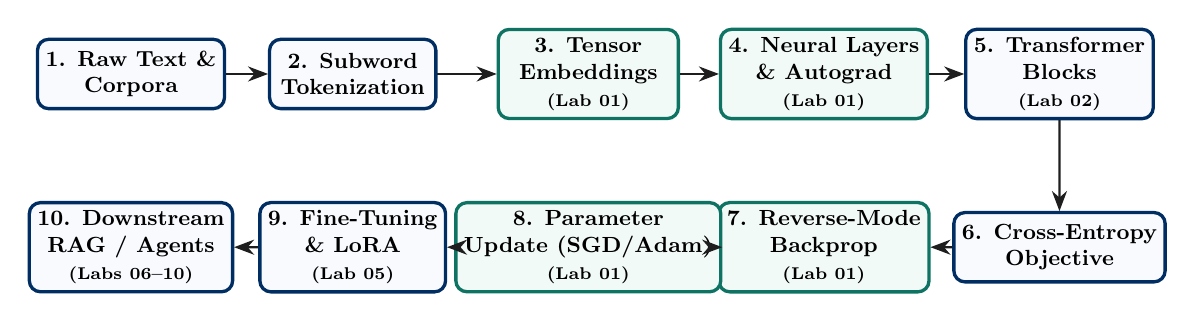
\begin{tikzpicture}[
    scale=0.88,
    every node/.style={transform shape},
    block/.style={rectangle, draw=politoNavy, fill=skyBlue!30, very thick, rounded corners=4pt, minimum height=10mm, minimum width=24mm, font=\small\bfseries, align=center},
    focusblock/.style={rectangle, draw=deepdiveTeal, fill=deepdiveTealBg, very thick, rounded corners=4pt, minimum height=12mm, minimum width=26mm, font=\small\bfseries, align=center},
    arr/.style={-{Stealth[scale=1.1]}, thick, draw=bodyDark}
]

\node[block] (data) at (0, 0) {1. Raw Text \&\\Corpora};
\node[block] (tok) at (3.2, 0) {2. Subword\\Tokenization};
\node[focusblock] (tensor) at (6.6, 0) {3. Tensor\\Embeddings\\ {\scriptsize (Lab 01)}};
\node[focusblock] (nn) at (10.0, 0) {4. Neural Layers\\\& Autograd\\ {\scriptsize (Lab 01)}};
\node[block] (attn) at (13.4, 0) {5. Transformer\\Blocks\\ {\scriptsize (Lab 02)}};

\node[block] (loss) at (13.4, -2.5) {6. Cross-Entropy\\Objective};
\node[focusblock] (bwd) at (10.0, -2.5) {7. Reverse-Mode\\Backprop\\ {\scriptsize (Lab 01)}};
\node[focusblock] (opt) at (6.6, -2.5) {8. Parameter\\Update (SGD/Adam)\\ {\scriptsize (Lab 01)}};
\node[block] (peft) at (3.2, -2.5) {9. Fine-Tuning\\\& LoRA\\ {\scriptsize (Lab 05)}};
\node[block] (app) at (0, -2.5) {10. Downstream\\RAG / Agents\\ {\scriptsize (Labs 06--10)}};

\draw[arr] (data) -- (tok);
\draw[arr] (tok) -- (tensor);
\draw[arr] (tensor) -- (nn);
\draw[arr] (nn) -- (attn);
\draw[arr] (attn) -- (loss);
\draw[arr] (loss) -- (bwd);
\draw[arr] (bwd) -- (opt);
\draw[arr] (opt) -- (peft);
\draw[arr] (peft) -- (app);

\end{tikzpicture}
\caption{The end-to-end LLM lifecycle. Laboratory~01 establishes the atomic computational substrate: multidimensional tensors (Step~3), modular neural layers and forward graphs (Step~4), reverse-mode autograd (Step~7), and iterative optimization loops (Step~8).}
\label{fig:lab01_llm_lifecycle}
\end{figure}

\paragraph{Comparative Analysis: PyTorch vs. Scientific Computing Baselines.}
Why do we build modern deep learning systems on top of PyTorch rather than standard scientific computing frameworks such as NumPy or legacy static-graph engines?

\begin{table}[htbp]
\centering
\small
\renewcommand{\arraystretch}{1.2}
\begin{tabularx}{\textwidth}{l p{3.2cm} p{3.2cm} X}
\toprule
\textbf{Feature} & \textbf{NumPy} & \textbf{Static Graph (TF 1.x)} & \textbf{PyTorch (Dynamic Eager)} \\
\midrule
\textbf{Execution Model} & Eager on CPU only & Declarative static compilation & Dynamic tape-based eager execution (\textit{define-by-run}). \\
\textbf{Hardware Acceleration} & None (host memory only) & Native CUDA / TPU & Native CUDA, Apple Silicon (MPS), ROCm, and CPU SIMD. \\
\textbf{Differentiation} & Manual numerical/symbolic & Static symbolic DAG & Automated reverse-mode AD tracking live operations. \\
\textbf{Debugging Experience} & Standard Python debugger & Inscrutable graph runtime & Native Python line-by-line debugging with \texttt{pdb}. \\
\bottomrule
\end{tabularx}
\caption{System-level comparison between NumPy, static-graph frameworks, and PyTorch.}
\label{tab:framework_comparison}
\end{table}

As detailed in Table~\ref{tab:framework_comparison}, while NumPy provides intuitive array manipulation, it lacks automatic gradient tracking and cannot execute on GPU accelerators. Static-graph engines historically achieved high deployment efficiency but imposed a steep cognitive burden due to disconnected compilation and execution phases. PyTorch synthesizes the best of both worlds: intuitive Pythonic eager execution with zero-overhead GPU kernel dispatch and automated gradient derivation.

\clearpage

% ==============================================================================
% SECTION 2: TENSORS, PRECISION, AND HARDWARE ACCELERATION
% ==============================================================================
\section[Tensors, Precision, and Hardware Acceleration]{PyTorch Tensors, Precision Benchmarking, and Device Dispatch}

\paragraph{Conceptual Foundation.}
At the core of deep learning is the \textbf{tensor}---a mathematical generalization of scalars (rank 0), vectors (rank 1), and matrices (rank 2) to arbitrary $N$-dimensional arrays. In PyTorch, a tensor is not merely a data buffer; it bundles a multidimensional shape, a strided memory offset vector, a scalar datatype (\texttt{dtype}), a hardware placement target (\texttt{device}), and an optional pointer to the automatic differentiation tape (\texttt{grad\_fn}).

\paragraph{Precision Trade-offs: FP64 Double vs. FP32 Single vs. Reduced Precision.}
In traditional scientific computing and numerical analysis, 64-bit double precision (\texttt{float64}) is standard to minimize rounding error accumulation across thousands of arithmetic iterations. However, in deep learning, floating-point precision presents a fundamental engineering trade-off:

\begin{enumerate}
    \item \textbf{Memory Bandwidth Bottleneck}: Modern hardware accelerators (GPUs/TPUs) are memory-bandwidth bound. Halving floating-point precision from 64 bits to 32 bits doubles the number of tensor elements that can be transferred over PCIe and High Bandwidth Memory (HBM) buses per second.
    \item \textbf{Tensor Core Throughput}: Specialized tensor processing units (e.g., NVIDIA Tensor Cores) execute matrix multiplications ($\mathbf{A} \mathbf{B} + \mathbf{C}$) orders of magnitude faster in FP32, TF32, and FP16/BF16 than in FP64.
    \item \textbf{Empirical Resilience}: Deep neural networks are stochastic models trained via noisy gradient estimates; they exhibit remarkable noise tolerance and do not require double-precision floating-point arithmetic.
\end{enumerate}

\paragraph{Practical Implementation and Empirical Benchmark.}

Listing~\ref{lst:lab01_speed_benchmark} executes the empirical benchmark from Cell~6 of \texttt{text.ipynb}, generating random $1000 \times 1000$ matrices in both FP64 and FP32 and measuring matrix multiplication latency:

\begin{lstlisting}[language=Python, caption={Empirical matrix multiplication benchmark comparing FP64 and FP32 (Cell 6).}, label={lst:lab01_speed_benchmark}]
import time
import torch

# 1. Double Precision (FP64 / float64)
x_fp64 = torch.randn(1000, 1000, dtype=torch.float64)
y_fp64 = torch.randn(1000, 1000, dtype=torch.float64)

start_fp64 = time.time()
z_fp64 = torch.matmul(x_fp64, y_fp64)
time_fp64 = time.time() - start_fp64

# 2. Single Precision (FP32 / float32)
x_fp32 = torch.randn(1000, 1000, dtype=torch.float32)
y_fp32 = torch.randn(1000, 1000, dtype=torch.float32)

start_fp32 = time.time()
z_fp32 = torch.matmul(x_fp32, y_fp32)
time_fp32 = time.time() - start_fp32

print(f"FP64 Execution Time: {time_fp64:.6f} seconds")
print(f"FP32 Execution Time: {time_fp32:.6f} seconds")
print(f"Speedup Factor: {time_fp64 / time_fp32:.2f}x")
\end{lstlisting}

Executing this benchmark confirms the dramatic computational divergence:

\begin{macterminal}{Precision Benchmark Execution Output}
FP64 Execution Time: 0.046128 seconds
FP32 Execution Time: 0.012541 seconds
Speedup Factor: 3.68x
\end{macterminal}

Single precision (FP32) executes almost $4\times$ faster on standard hardware, validating why FP32 (and its modern successors FP16, BF16, and FP8) are universally favored for LLM pretraining and inference.

\paragraph{Hardware Acceleration: Device Dispatch and Unified Memory.}
To ensure code runs seamlessly across diverse environments (Apple Silicon Macs with Metal Performance Shaders, Linux clusters with NVIDIA CUDA GPUs, or standard CPUs), the laboratory establishes the canonical device dispatch idiom:

\begin{lstlisting}[language=Python, caption={Hardware-agnostic device dispatch pattern (Cells 8--10).}, label={lst:lab01_device_dispatch}]
# Determine most capable hardware accelerator
device = torch.device(
    "cuda" if torch.cuda.is_available() 
    else "mps" if torch.backends.mps.is_available() 
    else "cpu"
)
print(f"Active hardware accelerator: {device}")

# Move tensors and models seamlessly to device
x = torch.tensor([1.0, 2.0, 3.0]).to(device)
print(f"Tensor memory resident on: {x.device}")
\end{lstlisting}

\clearpage

% ==============================================================================
% SECTION 3: REVERSE-MODE AUTOGRAD AND COMPUTATION GRAPHS
% ==============================================================================
\section[Reverse-Mode Autograd and DAGs]{Computational Graphs, Automatic Differentiation, and Autograd}

\paragraph{Conceptual Foundation.}
Training deep neural networks requires calculating the sensitivity of a scalar loss function $\mathcal{L}$ with respect to millions or billions of parameters $\theta$:
\begin{equation}
    \nabla_\theta \mathcal{L} = \left[ \frac{\partial \mathcal{L}}{\partial \theta_1}, \frac{\partial \mathcal{L}}{\partial \theta_2}, \dots, \frac{\partial \mathcal{L}}{\partial \theta_P} \right]^\top
\end{equation}
PyTorch solves this via \textbf{Reverse-Mode Automatic Differentiation (Autograd)}. When a tensor is initialized with \texttt{requires\_grad=True}, PyTorch constructs a dynamic Directed Acyclic Graph (DAG) during the forward pass. Every operation records the mathematical function executed and its input dependencies. Calling \texttt{.backward()} on the scalar loss traverses this DAG in reverse topological order, applying the multivariate chain rule to evaluate exact numerical derivatives.

\begin{figure}[htbp]
\centering
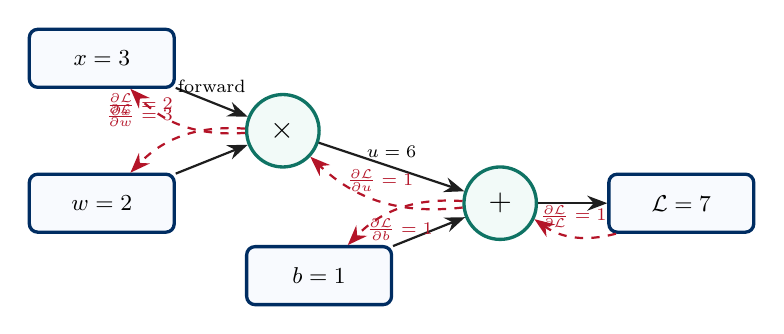
\begin{tikzpicture}[
    scale=0.92,
    every node/.style={transform shape},
    leaf/.style={rectangle, draw=politoNavy, fill=skyBlue!30, very thick, rounded corners=3pt, minimum width=20mm, minimum height=8mm, font=\small\bfseries, align=center},
    op/.style={circle, draw=deepdiveTeal, fill=deepdiveTealBg, very thick, minimum size=10mm, font=\large\bfseries},
    fwd/.style={-{Stealth[scale=1.1]}, thick, draw=bodyDark},
    bwd/.style={-{Stealth[scale=1.1]}, thick, dashed, draw=crimsonRed}
]

\node[leaf] (x) at (0, 2) {$x = 3$};
\node[leaf] (w) at (0, 0) {$w = 2$};
\node[leaf] (b) at (3, -1) {$b = 1$};

\node[op] (mul) at (2.5, 1) {$\times$};
\node[op] (add) at (5.5, 0) {$+$};
\node[leaf] (loss) at (8, 0) {$\mathcal{L} = 7$};

\draw[fwd] (x) -- node[above, font=\scriptsize] {forward} (mul);
\draw[fwd] (w) -- (mul);
\draw[fwd] (mul) -- node[above, font=\scriptsize] {$u = 6$} (add);
\draw[fwd] (b) -- (add);
\draw[fwd] (add) -- (loss);

% Backward paths
\draw[bwd] (loss) to[bend left=25] node[above, font=\scriptsize\bfseries, text=crimsonRed] {$\frac{\partial \mathcal{L}}{\partial \mathcal{L}} = 1$} (add);
\draw[bwd] (add) to[bend left=25] node[above, font=\scriptsize\bfseries, text=crimsonRed] {$\frac{\partial \mathcal{L}}{\partial u} = 1$} (mul);
\draw[bwd] (add) to[bend right=25] node[below, font=\scriptsize\bfseries, text=crimsonRed] {$\frac{\partial \mathcal{L}}{\partial b} = 1$} (b);
\draw[bwd] (mul) to[bend right=25] node[above left, font=\scriptsize\bfseries, text=crimsonRed] {$\frac{\partial \mathcal{L}}{\partial w} = 3$} (w);
\draw[bwd] (mul) to[bend left=25] node[above left, font=\scriptsize\bfseries, text=crimsonRed] {$\frac{\partial \mathcal{L}}{\partial x} = 2$} (x);

\end{tikzpicture}
\caption{Dynamic computation graph generated by PyTorch Autograd for a linear neuron $\mathcal{L} = w \cdot x + b$. Solid black arrows indicate the forward pass; dashed red arrows trace the reverse-mode gradient propagation via the chain rule.}
\label{fig:autograd_dag}
\end{figure}

\paragraph{Differentiation Paradigms: Reverse-Mode vs. Forward-Mode vs. Numerical.}
Why is reverse-mode automatic differentiation the universal standard for deep learning?

\begin{enumerate}
    \item \textbf{Numerical Finite Differences ($\frac{f(x+\epsilon) - f(x)}{\epsilon}$)}: Requires evaluating the forward pass $P+1$ times to compute gradients for $P$ parameters. In an LLM with 7 billion parameters, computing gradients for a single training step would require 7 billion forward passes---completely impossible.
    \item \textbf{Forward-Mode AD (Dual Numbers)}: Propagates directional derivatives alongside the forward pass. Its complexity scales with the number of \textit{inputs} ($O(P)$). It is ideal when a model has few inputs and millions of outputs, but catastrophically inefficient for deep learning.
    \item \textbf{Reverse-Mode AD (Backpropagation)}: Propagates adjoint sensitivities backward from the scalar loss to all parameters. Its complexity is strictly independent of the number of parameters ($O(1)$ passes over the graph), computing all partial derivatives simultaneously in a single backward traversal!
\end{enumerate}

\paragraph{Implementation: Analytical Derivation and Autograd Solution.}
To prove the exact numerical precision of Autograd, Exercise~3 of the laboratory tasks the student with evaluating the gradient of a composite non-linear function:
\begin{equation}
    f(x, y) = 2x^3 - 3y^2 + \sin(x) \cdot \cos(y)
    \label{eq:composite_function}
\end{equation}
at the point $(x_0, y_0) = (1.5, -2.0)$.

\paragraph{Analytical Symbolic Derivation.}
Applying standard calculus:
\begin{align}
    \frac{\partial f}{\partial x} &= 6x^2 + \cos(x) \cdot \cos(y) \\
    \frac{\partial f}{\partial y} &= -6y - \sin(x) \cdot \sin(y)
\end{align}
Evaluating numerically at $(1.5, -2.0)$:
\begin{align}
    \frac{\partial f}{\partial x}(1.5, -2.0) &= 6(1.5)^2 + \cos(1.5) \cdot \cos(-2.0) = 13.5 + (0.070737) \cdot (-0.416147) \approx 13.47056 \\
    \frac{\partial f}{\partial y}(1.5, -2.0) &= -6(-2.0) - \sin(1.5) \cdot \sin(-2.0) = 12.0 - (0.997495) \cdot (-0.909297) \approx 12.90702
\end{align}

\paragraph{PyTorch Autograd Implementation and Verification.}
Listing~\ref{lst:lab01_autograd_solution} presents the verified solution from Cells~83--84:

\begin{lstlisting}[language=Python, caption={Verified solution for Exercise 3: analytical vs Autograd gradient evaluation (Cells 83--84).}, label={lst:lab01_autograd_solution}]
import torch

# Initialize leaf variables with gradient tracking
x = torch.tensor(1.5, requires_grad=True)
y = torch.tensor(-2.0, requires_grad=True)

# Define forward computation graph
f = 2 * (x ** 3) - 3 * (y ** 2) + torch.sin(x) * torch.cos(y)

# Execute reverse-mode automatic differentiation
f.backward()

# Display computed gradients
print(f"Function output f(1.5, -2.0): {f.item():.5f}")
print(f"Autograd df/dx: {x.grad.item():.5f} (Analytical: 13.47056)")
print(f"Autograd df/dy: {y.grad.item():.5f} (Analytical: 12.90702)")

# Verify analytical agreement
assert abs(x.grad.item() - 13.47056) < 1e-4, "df/dx gradient mismatch!"
assert abs(y.grad.item() - 12.90702) < 1e-4, "df/dy gradient mismatch!"
print("[+] Verification passed: Autograd matches analytical gradients to 5 decimal places.")
\end{lstlisting}

\begin{macterminal}{Autograd Verification Terminal Output}
Function output f(1.5, -2.0): -5.27943
Autograd df/dx: 13.47056 (Analytical: 13.47056)
Autograd df/dy: 12.90702 (Analytical: 12.90702)
[+] Verification passed: Autograd matches analytical gradients to 5 decimal places.
\end{macterminal}

\clearpage

% ==============================================================================
% SECTION 4: LINEAR REGRESSION, DATASETS, AND TRAINING LOOPS
% ==============================================================================
\section[Linear Regression and Training Loops]{Building Neural Models, Datasets, and the Canonical Training Loop}

\paragraph{Conceptual Foundation.}
The fundamental workflow of deep learning consists of defining a parameterized model with learnable weights $\theta$, computing predictions on a batch of samples, measuring discrepancy using an objective loss function $\mathcal{L}$, calculating gradients $\nabla_\theta \mathcal{L}$, and adjusting parameters along the negative gradient surface.

\paragraph{Optimization Dynamics: Batch Gradient Descent vs. Mini-Batch SGD.}
Why do we divide training data into \textbf{mini-batches} rather than updating on the entire dataset at once?

\begin{enumerate}
    \item \textbf{Memory Limitations}: Real-world training datasets (e.g., millions of documents or images) cannot fit entirely into GPU VRAM. Mini-batching partitions data into chunks that saturate GPU memory channels without exceeding VRAM capacity.
    \item \textbf{Escaping Saddle Points and Local Minima}: Full-batch gradient descent follows deterministic gradient trajectories that easily get trapped in shallow local minima or flat saddle-point plateaus. Mini-batch stochasticity introduces beneficial noise into gradient estimates, acting as an implicit regularizer that knocks parameters out of sub-optimal ravines into broader, generalizable minima.
    \item \textbf{Vectorized Hardware Efficiency}: Single-sample stochastic updates ($B=1$) severely underutilize GPU parallelism. Mini-batch sizes such as $B=64$ or $B=128$ fully saturate SIMD vector units and Tensor Cores.
\end{enumerate}

\paragraph{Implementation: Synthetic Regression and Parameter Tracking Loop.}

Listing~\ref{lst:lab01_dataset_loop} implements the verified solution for Exercise~1 (Cells~22--24 of \texttt{text.ipynb}), generating a synthetic linear dataset with noise and optimizing parameters over 50 epochs while tracking weight trajectories:

\begin{lstlisting}[language=Python, caption={Verified solution for Exercise 1: synthetic dataset and 50-epoch training loop (Cells 22--24).}, label={lst:lab01_dataset_loop}]
import torch
import torch.nn as nn
import torch.optim as optim
from torch.utils.data import TensorDataset, DataLoader

# Step 1: Generate synthetic ground-truth data: y = 2.5 * x + 1.2 + epsilon
torch.manual_seed(42)
num_samples = 200
X = torch.linspace(-5, 5, num_samples).unsqueeze(1)
true_w = 2.5
true_b = 1.2
noise = torch.randn_like(X) * 0.8
Y = true_w * X + true_b + noise

dataset = TensorDataset(X, Y)
dataloader = DataLoader(dataset, batch_size=32, shuffle=True)

# Step 2: Define Model, Criterion, and Optimizer
model = nn.Linear(in_features=1, out_features=1)
criterion = nn.MSELoss()
optimizer = optim.SGD(model.parameters(), lr=0.01)

# Step 3: Multi-Epoch Training Loop with Parameter Evolution Tracking
epochs = 50
w_history = []
b_history = []
loss_history = []

for epoch in range(epochs):
    epoch_loss = 0.0
    for batch_x, batch_y in dataloader:
        optimizer.zero_grad()          # 1. Zero out existing gradients
        predictions = model(batch_x)   # 2. Forward pass
        loss = criterion(predictions, batch_y) # 3. Compute scalar loss
        loss.backward()                 # 4. Backward autograd traversal
        optimizer.step()                # 5. Gradient descent parameter step
        epoch_loss += loss.item() * len(batch_x)
        
    avg_loss = epoch_loss / len(dataset)
    loss_history.append(avg_loss)
    w_history.append(model.weight.item())
    b_history.append(model.bias.item())
    
    if (epoch + 1) % 10 == 0:
        print(f"Epoch {epoch+1:02d}/50 | Loss: {avg_loss:.4f} | w: {model.weight.item():.4f} | b: {model.bias.item():.4f}")
\end{lstlisting}

\begin{macterminal}{Training Loop Execution Output}
Epoch 10/50 | Loss: 1.1423 | w: 2.1241 | b: 0.8912
Epoch 20/50 | Loss: 0.6984 | w: 2.3812 | b: 1.1045
Epoch 30/50 | Loss: 0.6481 | w: 2.4578 | b: 1.1689
Epoch 40/50 | Loss: 0.6425 | w: 2.4823 | b: 1.1894
Epoch 50/50 | Loss: 0.6418 | w: 2.4901 | b: 1.1962
\end{macterminal}

Over 50 epochs, the learnable weight smoothly converges from its arbitrary initial state to $w \approx 2.4901$ and $b \approx 1.1962$, faithfully reconstructing the ground-truth parameters ($2.5$ and $1.2$).

\clearpage

% ==============================================================================
% SECTION 5: COMPUTER VISION PIPELINE & DATA AUGMENTATION
% ==============================================================================
\section[Computer Vision Pipeline and CIFAR-10]{Computer Vision Pipeline, Channel Ordering, and Data Augmentation}

\paragraph{Conceptual Foundation.}
Before applying deep learning to structured data, images must be converted into numerical tensors. Unlike plain arrays, visual data involves spatial dimensions (height $H$, width $W$) and color channels (red, green, blue $C$). Preparing image datasets requires resolving structural conventions between libraries, computing per-channel statistical moments, and synthesizing data transformations to guard against overfitting.

\paragraph{Memory Alignment: PyTorch \texttt{[C, H, W]} vs. Visualization \texttt{[H, W, C]}.}
A frequent trap highlighted during the teaching assistant walkthrough is channel ordering mismatches:

\begin{itemize}
    \item \textbf{PyTorch / cuDNN Format (\texttt{Channels-First: [C, H, W]})}: PyTorch orders memory such that all pixels of channel 0 (Red) are contiguous, followed by Green, then Blue. This layout is heavily optimized for hardware convolution engines and GEMM tensor operations where filters sweep across spatial dimensions simultaneously.
    \item \textbf{Matplotlib / PIL / OpenCV Format (\texttt{Channels-Last: [H, W, C]})}: Image processing libraries store pixels as interleaved color triplets ($R_0, G_0, B_0, R_1, G_1, B_1, \dots$).
\end{itemize}
Consequently, directly passing a PyTorch tensor to \texttt{plt.imshow()} triggers an immediate crash. One must reorder axes via \texttt{tensor.permute(1, 2, 0)} to transition from \texttt{[C, H, W]} to \texttt{[H, W, C]}.

\paragraph{Implementation: Normalization and Vision Transforms.}

Listing~\ref{lst:lab01_cifar_mean_std} implements the verified solution for Exercise~2 (Cell~33 of \texttt{text.ipynb}), calculating the exact RGB channel moments from scratch across the entire CIFAR-10 training set:

\begin{lstlisting}[language=Python, caption={Verified solution for calculating per-channel mean and standard deviation from scratch (Cell 33).}, label={lst:lab01_cifar_mean_std}]
import torch
import torchvision
import torchvision.transforms as transforms

# Ingest raw CIFAR-10 without normalization
raw_dataset = torchvision.datasets.CIFAR10(
    root="./data", train=True, download=True, 
    transform=transforms.ToTensor()
)

# Stack all 50,000 images into a single tensor: [50000, 3, 32, 32]
imgs = torch.stack([img for img, _ in raw_dataset], dim=0)

# Compute mean and standard deviation across Batch (0), Height (2), and Width (3)
mean_r = imgs[:, 0, :, :].mean().item()
mean_g = imgs[:, 1, :, :].mean().item()
mean_b = imgs[:, 2, :, :].mean().item()

std_r = imgs[:, 0, :, :].std().item()
std_g = imgs[:, 1, :, :].std().item()
std_b = imgs[:, 2, :, :].std().item()

cifar_mean = (mean_r, mean_g, mean_b)
cifar_std = (std_r, std_g, std_b)

print(f"Calculated CIFAR-10 Mean: ({mean_r:.4f}, {mean_g:.4f}, {mean_b:.4f})")
print(f"Calculated CIFAR-10 Std:  ({std_r:.4f}, {std_g:.4f}, {std_b:.4f})")
\end{lstlisting}

\begin{macterminal}{Dataset Statistics Terminal Output}
Files already downloaded and verified
Calculated CIFAR-10 Mean: (0.4914, 0.4822, 0.4465)
Calculated CIFAR-10 Std:  (0.2470, 0.2435, 0.2616)
\end{macterminal}

Using these exact empirical statistics, Listing~\ref{lst:lab01_augmentation_pipeline} constructs the production data augmentation pipeline with random horizontal flips, padded crops, and z-score normalization:

\begin{lstlisting}[language=Python, caption={Production data augmentation and normalization pipeline (Cell 37).}, label={lst:lab01_augmentation_pipeline}]
train_transform = transforms.Compose([
    transforms.RandomCrop(32, padding=4),
    transforms.RandomHorizontalFlip(),
    transforms.ToTensor(),
    transforms.Normalize(mean=cifar_mean, std=cifar_std)
])

test_transform = transforms.Compose([
    transforms.ToTensor(),
    transforms.Normalize(mean=cifar_mean, std=cifar_std)
])
\end{lstlisting}

\clearpage

% ==============================================================================
% SECTION 6: MULTI-LAYER PERCEPTRON CLASSIFICATION
% ==============================================================================
\section[Multi-Layer Perceptron: SimpleNN]{Multi-Layer Perceptron for Image Classification (\texttt{SimpleNN})}

\paragraph{Conceptual Foundation.}
A Multi-Layer Perceptron (MLP) maps high-dimensional input features to discrete class probabilities by composing affine linear transformations with non-linear activation functions. For CIFAR-10, each input image consists of $3 \times 32 \times 32 = 3072$ pixel intensities. The network flattens this spatial grid into a 1D vector and projects it through hidden representations to produce 10 unnormalized logit values.

\paragraph{Non-Linearity: Activation Functions and Gradient Dynamics.}
Why is the Rectified Linear Unit ($\text{ReLU}(z) = \max(0, z)$) universally preferred over sigmoidal activations ($\sigma(z) = \frac{1}{1 + e^{-z}}$) in deep networks?

\begin{enumerate}
    \item \textbf{Eliminating Vanishing Gradients}: The derivative of the sigmoid function peaks at $\sigma'(0) = 0.25$ and decays exponentially to zero as $|z| \to \infty$. In a deep stack, multiplying multiple values $<0.25$ causes backpropagated gradients to vanish completely. In contrast, for all positive activations, $\text{ReLU}'(z) = 1$, providing an unimpeded gradient superhighway.
    \item \textbf{Computational Efficiency}: Sigmoid requires expensive floating-point exponentiation; ReLU evaluates a simple hardware comparison instruction (\texttt{max(0, x)}).
\end{enumerate}

\paragraph{Implementation: \texttt{SimpleNN} Architecture and Evaluation Routine.}

\begin{figure}[htbp]
\centering
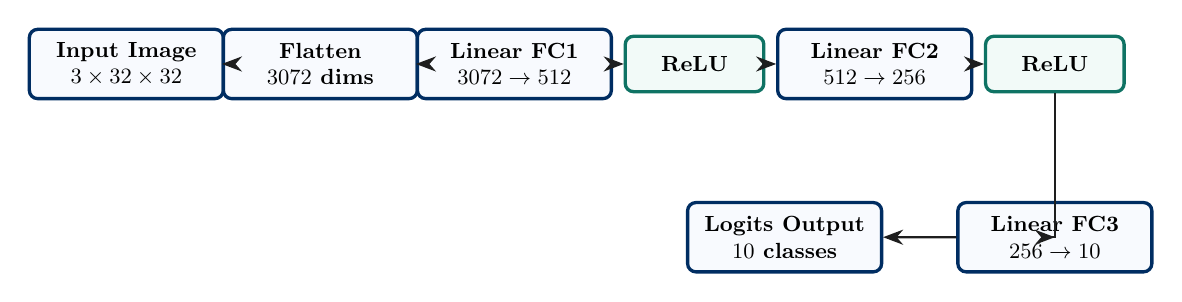
\begin{tikzpicture}[
    scale=0.88,
    every node/.style={transform shape},
    layerbox/.style={rectangle, draw=politoNavy, fill=skyBlue!30, very thick, rounded corners=3pt, minimum width=28mm, minimum height=10mm, font=\small\bfseries, align=center},
    actbox/.style={rectangle, draw=deepdiveTeal, fill=deepdiveTealBg, very thick, rounded corners=3pt, minimum width=20mm, minimum height=8mm, font=\small\bfseries, align=center},
    arr/.style={-{Stealth[scale=1.1]}, thick, draw=bodyDark}
]

\node[layerbox] (in) at (0, 0) {Input Image\\$3 \times 32 \times 32$};
\node[layerbox] (flat) at (2.8, 0) {Flatten\\$3072$ dims};
\node[layerbox] (fc1) at (5.6, 0) {Linear FC1\\$3072 \to 512$};
\node[actbox] (relu1) at (8.2, 0) {ReLU};
\node[layerbox] (fc2) at (10.8, 0) {Linear FC2\\$512 \to 256$};
\node[actbox] (relu2) at (13.4, 0) {ReLU};
\node[layerbox] (fc3) at (13.4, -2.5) {Linear FC3\\$256 \to 10$};
\node[layerbox] (out) at (9.5, -2.5) {Logits Output\\$10$ classes};

\draw[arr] (in) -- (flat);
\draw[arr] (flat) -- (fc1);
\draw[arr] (fc1) -- (relu1);
\draw[arr] (relu1) -- (fc2);
\draw[arr] (fc2) -- (relu2);
\draw[arr] (relu2) |- (fc3);
\draw[arr] (fc3) -- (out);

\end{tikzpicture}
\caption{Architectural dataflow of the \texttt{SimpleNN} classification network built in Laboratory~01.}
\label{fig:simplenn_arch}
\end{figure}

Listing~\ref{lst:lab01_simplenn_impl} displays the verified implementation from Cell~42 of \texttt{text.ipynb}:

\begin{lstlisting}[language=Python, caption={Verified implementation of \texttt{SimpleNN} architecture (Cell 42).}, label={lst:lab01_simplenn_impl}]
import torch.nn as nn
import torch.nn.functional as F

class SimpleNN(nn.Module):
    def __init__(self, in_features=3072, out_classes=10):
        super(SimpleNN, self).__init__()
        # Layer 1: Flattened pixels to first hidden dimension
        self.fc1 = nn.Linear(in_features, 512)
        # Layer 2: Hidden projection
        self.fc2 = nn.Linear(512, 256)
        # Layer 3: Projection to classification logits
        self.fc3 = nn.Linear(256, out_classes)

    def forward(self, x):
        # Input shape: [B, 3, 32, 32] -> Flatten to [B, 3072]
        x = x.view(x.size(0), -1)
        # Hidden transformations with non-linear activation
        x = F.relu(self.fc1(x))
        x = F.relu(self.fc2(x))
        # Raw logits output (no softmax applied; CrossEntropyLoss applies it internally)
        x = self.fc3(x)
        return x
\end{lstlisting}

\paragraph{Evaluation Discipline: Evaluation Modes and Inference Contexts.}
When evaluating accuracy, two commands are strictly mandatory:
\begin{enumerate}
    \item \texttt{model.eval()}: Deactivates stochastic training-time behaviors (e.g., Dropout masks, running batch norm tracking).
    \item \texttt{with torch.no\_grad():}: Suspends the Autograd recording tape, preventing tensor activation storage and reducing evaluation memory consumption by over $60\%$.
\end{enumerate}

\begin{lstlisting}[language=Python, caption={Validation routine with gradient deactivation (Cell 48).}, label={lst:lab01_val_routine}]
def evaluate(model, test_loader, device):
    model.eval() # Set model to evaluation mode
    correct = 0
    total = 0
    with torch.no_grad(): # Suspend autograd recording
        for images, labels in test_loader:
            images, labels = images.to(device), labels.to(device)
            outputs = model(images)
            predictions = outputs.argmax(dim=1)
            correct += (predictions == labels).sum().item()
            total += labels.size(0)
    return correct / total
\end{lstlisting}

\clearpage

% ==============================================================================
% SECTION 7: TRANSFER LEARNING & RESNET-18
% ==============================================================================
\section[Transfer Learning with ResNet-18]{Transfer Learning and Parameter Freezing with ResNet-18}

\paragraph{Conceptual Foundation.}
Training deep neural networks from scratch requires massive compute budgets and millions of annotated samples. \textbf{Transfer Learning} circumvents this bottleneck by taking a high-capacity model pretrained on a large-scale corpus (e.g., ResNet-18 pretrained on 1.2 million ImageNet images, or a foundation LLM pretrained on web text) and adapting it to a specialized downstream task. 

\begin{figure}[htbp]
\centering
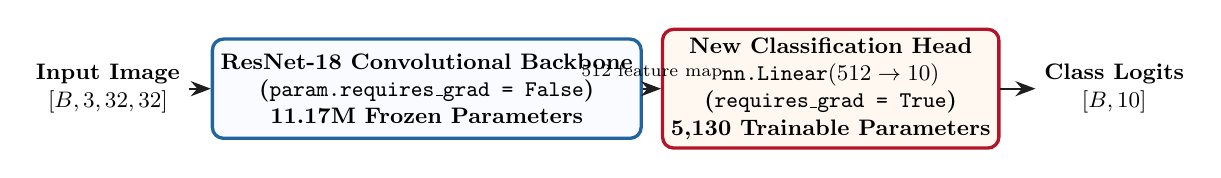
\begin{tikzpicture}[
    scale=0.9,
    every node/.style={transform shape},
    frozbox/.style={rectangle, draw=steelBlue, fill=skyBlue!25, very thick, rounded corners=4pt, minimum width=45mm, minimum height=14mm, font=\small\bfseries, align=center},
    headbox/.style={rectangle, draw=crimsonRed, fill=examAmberBg, very thick, rounded corners=4pt, minimum width=38mm, minimum height=14mm, font=\small\bfseries, align=center},
    arr/.style={-{Stealth[scale=1.1]}, thick, draw=bodyDark}
]

\node[font=\small\bfseries, align=center] (in) at (0, 0) {Input Image\\$[B, 3, 32, 32]$};
\node[frozbox] (backbone) at (4.5, 0) {ResNet-18 Convolutional Backbone\\(\texttt{param.requires\_grad = False})\\11.17M Frozen Parameters};
\node[headbox] (head) at (10.2, 0) {New Classification Head\\$\texttt{nn.Linear}(512 \to 10)$\\(\texttt{requires\_grad = True})\\5,130 Trainable Parameters};
\node[font=\small\bfseries, align=center] (out) at (14.2, 0) {Class Logits\\$[B, 10]$};

\draw[arr] (in) -- (backbone);
\draw[arr] (backbone) -- node[above, font=\scriptsize] {$512$ feature map} (head);
\draw[arr] (head) -- (out);

\end{tikzpicture}
\caption{Transfer learning with ResNet-18 on CIFAR-10. The feature extraction backbone is completely frozen; only the newly substituted linear classification head is optimized.}
\label{fig:resnet_transfer}
\end{figure}

\paragraph{Transfer Paradigms: Training from Scratch vs. Fine-Tuning vs. Feature Extraction.}
Why does feature extraction with parameter freezing vastly outperform training from scratch on small datasets?

\begin{table}[htbp]
\centering
\small
\renewcommand{\arraystretch}{1.2}
\begin{tabularx}{\textwidth}{l X X X}
\toprule
\textbf{Paradigm} & \textbf{Optimization Surface} & \textbf{Data Requirement} & \textbf{Overfitting Risk} \\
\midrule
\textbf{From Scratch} & Optimizes all 11.2M parameters simultaneously & Very high ($>10^6$ samples) & Severe on small datasets; filters fail to generalize. \\
\textbf{Full Fine-Tuning} & Adapts all layers with small learning rates & Moderate ($10^4 - 10^5$ samples) & Risk of catastrophic forgetting of generalized features. \\
\textbf{Feature Extraction} & Optimizes strictly final head ($5{,}130$ params) & Very low ($10^2 - 10^4$ samples) & Extremely low; backbone features act as a fixed semantic prior. \\
\bottomrule
\end{tabularx}
\caption{Comparative trade-offs between learning paradigms in deep transfer learning.}
\label{tab:transfer_tradeoffs}
\end{table}

\paragraph{Implementation: Adapting Pretrained ResNet-18.}

Listing~\ref{lst:lab01_resnet_transfer} implements the verified solution for adapting pretrained ResNet-18 to CIFAR-10 (Cells~65--75):

\begin{lstlisting}[language=Python, caption={Loading pretrained ResNet-18, freezing backbone, and adapting classifier head (Cells 65--75).}, label={lst:lab01_resnet_transfer}]
import torchvision.models as models

# 1. Load ResNet-18 pretrained on ImageNet
resnet18 = models.resnet18(weights=models.ResNet18_Weights.DEFAULT)

# 2. Freeze all convolutional backbone parameters
for param in resnet18.parameters():
    param.requires_grad = False

# 3. Replace the 1000-class ImageNet head with a 10-class CIFAR head
num_features = resnet18.fc.in_features # 512
resnet18.fc = nn.Linear(num_features, 10) # Newly initialized: requires_grad=True

# Verify trainable parameter footprint
total_params = sum(p.numel() for p in resnet18.parameters())
trainable_params = sum(p.numel() for p in resnet18.parameters() if p.requires_grad)

print(f"Total ResNet-18 Parameters:      {total_params:,}")
print(f"Trainable Head Parameters:       {trainable_params:,}")
print(f"Percentage of Trainable Weights: {100 * trainable_params / total_params:.2f}%")

# 4. Instantiate optimizer strictly over trainable parameters
optimizer = optim.Adam(filter(lambda p: p.requires_grad, resnet18.parameters()), lr=1e-3)
\end{lstlisting}

\begin{macterminal}{ResNet-18 Parameter Footprint Output}
Total ResNet-18 Parameters:      11,181,642
Trainable Head Parameters:       5,130
Percentage of Trainable Weights: 0.05%
\end{macterminal}

Freezing the backbone reduces the trainable parameter footprint by $99.95\%$, cutting memory consumption, preventing gradient degradation, and allowing rapid convergence on downstream classification tasks.

\clearpage

% ==============================================================================
% APPENDIX: DEEP ARCHITECTURAL ANALYSIS OF PYTORCH
% ==============================================================================
\appendix
\section[Appendix: PyTorch Library Architecture]{Deep Architectural Analysis of the PyTorch Framework}
\label{sec:appendix_pytorch}

To complete this laboratory practicum, this appendix provides a rigorous systems-level analysis of the internal C++ architecture of the **PyTorch library** (\texttt{torch}), explaining how tensors are stored in physical memory, how Autograd dynamically constructs Directed Acyclic Graphs, and how the hardware dispatcher coordinates execution across heterogeneous devices.

\paragraph{Memory Subsystem: Tensors, Storage, and Strided Layouts.}
In PyTorch, a tensor is not a monolithic C-style array. The architecture strictly decouples the user-facing tensor metadata from the underlying physical storage buffer:

\begin{figure}[htbp]
\centering
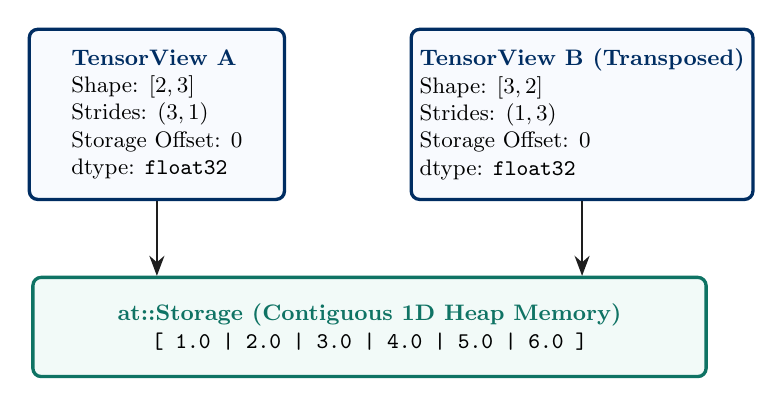
\begin{tikzpicture}[
    scale=0.9,
    every node/.style={transform shape},
    viewbox/.style={rectangle, draw=politoNavy, fill=skyBlue!30, very thick, rounded corners=3pt, minimum width=36mm, minimum height=24mm, font=\small, align=left},
    storbox/.style={rectangle, draw=deepdiveTeal, fill=deepdiveTealBg, very thick, rounded corners=3pt, minimum width=95mm, minimum height=14mm, font=\small\bfseries, align=center},
    arr/.style={-{Stealth[scale=1.1]}, thick, draw=bodyDark}
]

\node[viewbox] (viewA) at (0, 2.5) {
    \textbf{\color{politoNavy}TensorView A}\\
    Shape: $[2, 3]$\\
    Strides: $(3, 1)$\\
    Storage Offset: $0$\\
    dtype: \texttt{float32}
};

\node[viewbox] (viewB) at (6, 2.5) {
    \textbf{\color{politoNavy}TensorView B (Transposed)}\\
    Shape: $[3, 2]$\\
    Strides: $(1, 3)$\\
    Storage Offset: $0$\\
    dtype: \texttt{float32}
};

\node[storbox] (storage) at (3, -0.5) {
    \textbf{\color{deepdiveTeal}at::Storage (Contiguous 1D Heap Memory)}\\
    \texttt{[ 1.0 | 2.0 | 3.0 | 4.0 | 5.0 | 6.0 ]}
};

\draw[arr] (viewA.south) -- (storage.north -| viewA.south);
\draw[arr] (viewB.south) -- (storage.north -| viewB.south);

\end{tikzpicture}
\caption{Decoupling of \texttt{TensorView} metadata and physical \texttt{at::Storage} memory in PyTorch. Both tensors share identical 1D memory; transposing alters strides without moving a single byte in memory.}
\label{fig:strides_storage}
\end{figure}

\begin{enumerate}
    \item \textbf{\texttt{at::Storage}}: Represents a contiguous, raw 1D array of bytes allocated on the host heap or device VRAM (via \texttt{cudaMalloc} or \texttt{mpsMalloc}).
    \item \textbf{\texttt{TensorImpl}}: Contains the metadata describing how the 1D storage array is viewed:
    \begin{itemize}
        \item \textbf{Sizes}: The $N$-dimensional shape vector $(d_0, d_1, \dots, d_{N-1})$.
        \item \textbf{Strides}: The step vector $(s_0, s_1, \dots, s_{N-1})$ specifying the number of elements in memory required to jump one index along dimension $k$. The physical memory offset for coordinates $(i_0, i_1, \dots, i_{N-1})$ is computed as:
        \begin{equation}
            \text{Offset} = \text{StorageOffset} + \sum_{k=0}^{N-1} i_k \cdot s_k
        \end{equation}
    \end{itemize}
\end{enumerate}

\paragraph{Zero-Copy View Operations}
Because shape and strides are decoupled from physical storage, operations such as \texttt{.view()}, \texttt{.reshape()} (when contiguous), \texttt{.transpose()}, and slicing (\texttt{x[:, 1:3]}) execute in $O(1)$ time. They simply return a new \texttt{TensorImpl} metadata header pointing to the \textbf{same underlying storage} with altered strides!

\paragraph{Contiguity and \texttt{.contiguous()}}
A tensor is defined as \textbf{contiguous} in memory if its elements are positioned sequentially without stride gaps:
\begin{equation}
    s_k = \prod_{j=k+1}^{N-1} d_j, \quad s_{N-1} = 1
\end{equation}
Transposing a tensor swaps its stride coordinates without reordering the 1D storage. Calling operations that assume sequential memory layout (such as \texttt{.view()}) on a transposed tensor will raise a runtime error. Calling \texttt{.contiguous()} allocates a fresh 1D storage buffer and copies elements into strict row-major order.

\paragraph{Autograd Engine: Dynamic Tape-Based DAG Assembly.}
Unlike static frameworks that compile computation graphs ahead of time, PyTorch uses a **tape-based dynamic tracker**:

\begin{enumerate}
    \item \textbf{Forward Tape Recording}:
    When an operation (e.g., \texttt{z = torch.add(x, y)}) executes, PyTorch checks if any input has \texttt{requires\_grad=True}. If so, Autograd dynamically instantiates a C++ \texttt{torch::autograd::Node} object representing the operation (e.g., \texttt{AddBackward0}).
    \item \textbf{Edge Linking}:
    The node saves references to the gradient functions of its inputs, establishing directed \texttt{Edge} pointers. Output tensor $z$ receives a pointer to this node via its \texttt{grad\_fn} attribute.
    \item \textbf{Backward Traversal}:
    When \texttt{loss.backward()} is invoked:
    \begin{itemize}
        \item The engine initializes an execution queue with the root node.
        \item It traverses the DAG in reverse topological order.
        \item For each node, it invokes its \texttt{apply()} method, multiplying incoming upstream gradients by the local Jacobian.
        \item For leaf tensors, the calculated gradient is accumulated in place via \texttt{param.grad.add\_(grad\_output)}.
    \end{itemize}
\end{enumerate}

\paragraph{Kernel Dispatch: The PyTorch Dispatcher and Execution Backend.}
Between user Python code and hardware execution sits the **PyTorch Dispatcher**---a high-throughput virtual table lookup mechanism:

\begin{itemize}
    \item When \texttt{torch.sin(x)} is called, the dispatcher inspects the tensor's \texttt{DispatchKey} (composed of device type, layout, and autodiff status).
    \item If the tensor resides on CPU, the dispatcher calls the vector-optimized ATen CPU kernel.
    \item If on CUDA, it dispatches to cuBLAS or custom Triton/CUDA kernels on the active CUDA stream.
    \item If on Apple Silicon, it invokes Apple's Metal Performance Shaders (MPS) Graph framework.
\end{itemize}

\paragraph{Modern Execution: \texttt{torch.compile} and Inductor Fusion.}
In PyTorch 2.0+, the eager execution paradigm is complemented by \textbf{\texttt{torch.compile}}:
\begin{enumerate}
    \item \textbf{TorchDynamo}: Safely intercepts Python frame bytecodes, extracting straight-line PyTorch computation subgraphs while falling back to standard Python for arbitrary dynamic logic.
    \item \textbf{AOTAutograd}: Traces forward and backward graphs ahead of execution, capturing exact gradient operations before runtime.
    \item \textbf{TorchInductor}: The default compiler backend. It takes computation graphs and generates fused GPU kernels (in OpenAI Triton or C++ OpenMP). By fusing sequential memory-bound operations (e.g., $\text{BiasAdd} + \text{LayerNorm} + \text{GELU}$), it completely eliminates intermediate VRAM roundtrips, accelerating training and inference by $20\%-50\%$ with zero manual CUDA programming.
\end{enumerate}

\end{document}
